\documentclass[final,hyperref={pdfpagelabels=false}]{beamer}
\mode<presentation>{\usetheme{I6pd2}}
\usepackage[english]{babel}
\usepackage{amsmath,amsthm, amssymb, latexsym}
\usepackage[orientation=lanscape,size=a1,debug,scale=1.2]{beamerposter}
\usepackage{xcolor,colortbl}
\usepackage{tipa}
\usepackage{natbib}
\usepackage{multirow}
\usepackage{subfig}
\usepackage{tikz}
\usetikzlibrary{calc}
\usetikzlibrary{scopes}

%\usepackage{grffile}
%\usefonttheme[onlymath]{serif}
%\boldmath
% change list indention level
% \setdefaultleftmargin{3em}{}{}{}{}{}

\bibpunct[:]{(}{)}{,}{a}{}{,}
\newcommand{\ipa}[1]{\textipa{#1}} 

\usepackage{snapshot} % will write a .dep file with all dependencies, allows for easy bundling

\usepackage{array,booktabs,tabularx}
\newcolumntype{Z}{>{\centering\arraybackslash}X} % centered tabularx columns
\newcommand{\pphantom}{\textcolor{ta3aluminium}} % phantom introduces a vertical space in p formatted table columns??!!
\listfiles

%%%%
%%%%%%
\makeatletter
\define@key{beamerframe}{t}[true]{% top
  \beamer@frametopskip=.2cm plus .5\paperheight\relax%
  \beamer@framebottomskip=0pt plus 1fill\relax%
  \beamer@frametopskipautobreak=\beamer@frametopskip\relax%
  \beamer@framebottomskipautobreak=\beamer@framebottomskip\relax%
% \def\beamer@initfirstlineunskip{%
%   \def\beamer@firstlineitemizeunskip{%
%     \vskip-\partopsep\vskip-\topsep\vskip-\parskip%
%     \global\let\beamer@firstlineitemizeunskip=\relax}%
%   \everypar{\global\let\beamer@firstlineitemizeunskip=\relax}}
  \def\beamer@initfirstlineunskip{}%
}
\makeatother

\graphicspath{{figures/}}
 
\title{\huge Automating Acoustic and Articulatory Segmentation Exercises}
\author{Pertti Palo$^{\mathrm{a}}$}
\newcommand{\emails}{$^{\mathrm{a}}$pertti.palo@taurlin.org}
\institute{University of Alberta, Edmonton, Alberta, Canada}
\date{27th June 2026}

\newlength{\columnheight}
\setlength{\columnheight}{105cm}

\newcommand{\kommentti}[1]{{\bf[#1]}}


\begin{document}

\begin{frame}{} 
  \vspace{-1cm}
  \begin{columns}[t]
    \begin{column}{.4\linewidth}
      
      \begin{block}{Background: Phonetic Segmentation}
            \begin{itemize}
            \item Segmenting audio data has been part of our phonetic analysis
            toolset since the invention of audio recordings. 
            \item Since then we have gained two large improvements: 
            \begin{itemize}
              \item spectrograms \citep{Gabor-TheoryCommunicationPart-1946,KoenigEtAl-SoundSpectrograph-1946,Fant-SoundSpectrography-1961} and
              \item computer aided segmentation with programs such as Praat
                \citep{BoersmaWeenink-PraatDoingPhonetics-2010}. 
            \end{itemize}
            \item Segmentation has become more complex with the introduction of
              articulatory recording methods and other multimodal data, and the
              need to analyse them in conjunction with traditional audio
              recordings. 
            \item Now we are on the cusp of yet another great shift in how we
              work with the rapid improvement of forced alignment systems which
              started already before the current revolution in deep learning
              \citep[see e.g.][]{RosenfelderEtAl-FAVEForcedAlignment-2022} and is
              now becoming part of that revolution
              \citep{McAuliffeEtAl-MontrealForcedAligner-2017,KelleyEtAl-MasonAlbertaPhoneticSegmenter-2024}.
            \end{itemize}
      \end{block}
      
      \begin{block}{Purpose: Teach Segmentation with Minimal Effort}
        \begin{itemize}
        \item On the surface it might seem that the days of us needing to do
          manual segmentation are coming to an end, but we still need expert human
          segmenters for two crucial tasks:
        \begin{enumerate}
          \item The deep learning frameworks need data to learn from and
            this data needs to be well matched with what ever dataset we wish to
            eventually analyse.
          \item Even if it should happen that we get a magical large
            segmentation model that can deal with any human language and any
            dialect and accent there of -- even ones that do not exist yet -- we
            will still need to verify the output of any such model.
        \end{enumerate}
        \item In addition we are getting more and more time domain articulatory
        data. 
        \item Learning to segment data helps students develop an understanding
          of the concepts of phoneme and phone.
        \item Yet, surprisingly, we do not have easy methods for teaching
          segmentation to new learners -- neither for generating exercises nor
          for running them.
        \end{itemize}
      \end{block}

      \begin{block}{Method: Automated Exercises}
        \begin{itemize}
        \item A potential solution for this problem is generating segmentation
          exercises from existing data:
        \begin{itemize}
          \item Take any Praat TextGrids and the
            corresponding data -- whether audio only or multimodal -- and
            scramble the boundary placement within the TextGrid.
          \item Then let the learner correct the boundaries and compare to the
            original as they go along.
        \end{itemize} 
        \item This all has been implemented in PATKIT -- Phonetic Analysis
          ToolKIT \citep{PaloEtAl-PATKITPhoneticAnalysis-2026}.
        \item PATKIT has been written in the Python programming language.
        \item It can also process articulatory data.
        \item Get PATKIT on PyPi: \url{https://pypi.org/project/patkit/} or \\
        fork it on GitHub: \url{https://github.com/giuthas/patkit}.
        % \item Future versions are planned to include feedback on progress and
        %   accuracy, and the possibility to annotate boundaries and recordings
        %   with written notes.
        \end{itemize}
        % \vspace*{.5cm}
        % \begin{center}
        %   \input{figures/OD_vs_AAI.tex}
        % \end{center}
      \end{block}

      \begin{block}{Discussion: Future work}

        \begin{itemize}
        % \item This is where I need your help.
        \item I would like to know what you need.
        \item If you wish to contribute ideas, feature requests, bug reports,
        documentation, more exercises, code, or something else it would all be
        welcome.
        \end{itemize}
      \end{block}

      \begin{block}{References}

        \footnotesize
        % This needs to be replaced by a symlink or a fresh copy.
        \bibliography{main.bib}
        \bibliographystyle{apalike}

      \end{block}

      % \begin{block}{Acknowledgements}
      %   %\footnotesize
      %   \begin{minipage}{0.5\textwidth}
      %     % \includegraphics[scale=1]{figures/rbo.jpg}
      %     We wish to thank Steve Cowen for assistance with the
      %     ultrasound recordings and Professor Alan Wrench for advice
      %     and help with using AAA.
      %   \end{minipage}
      %   % \begin{minipage}{0.5\textwidth}
      %   %   \hspace{10cm}\includegraphics[height=3.5cm]{figures/CASL_Sub_logo.jpg} 
      %   % \end{minipage}
      % \end{block}
    \end{column}

    \begin{column}{.58\linewidth}
          
      \begin{block}{User interface: Example Answer}
          \centering
          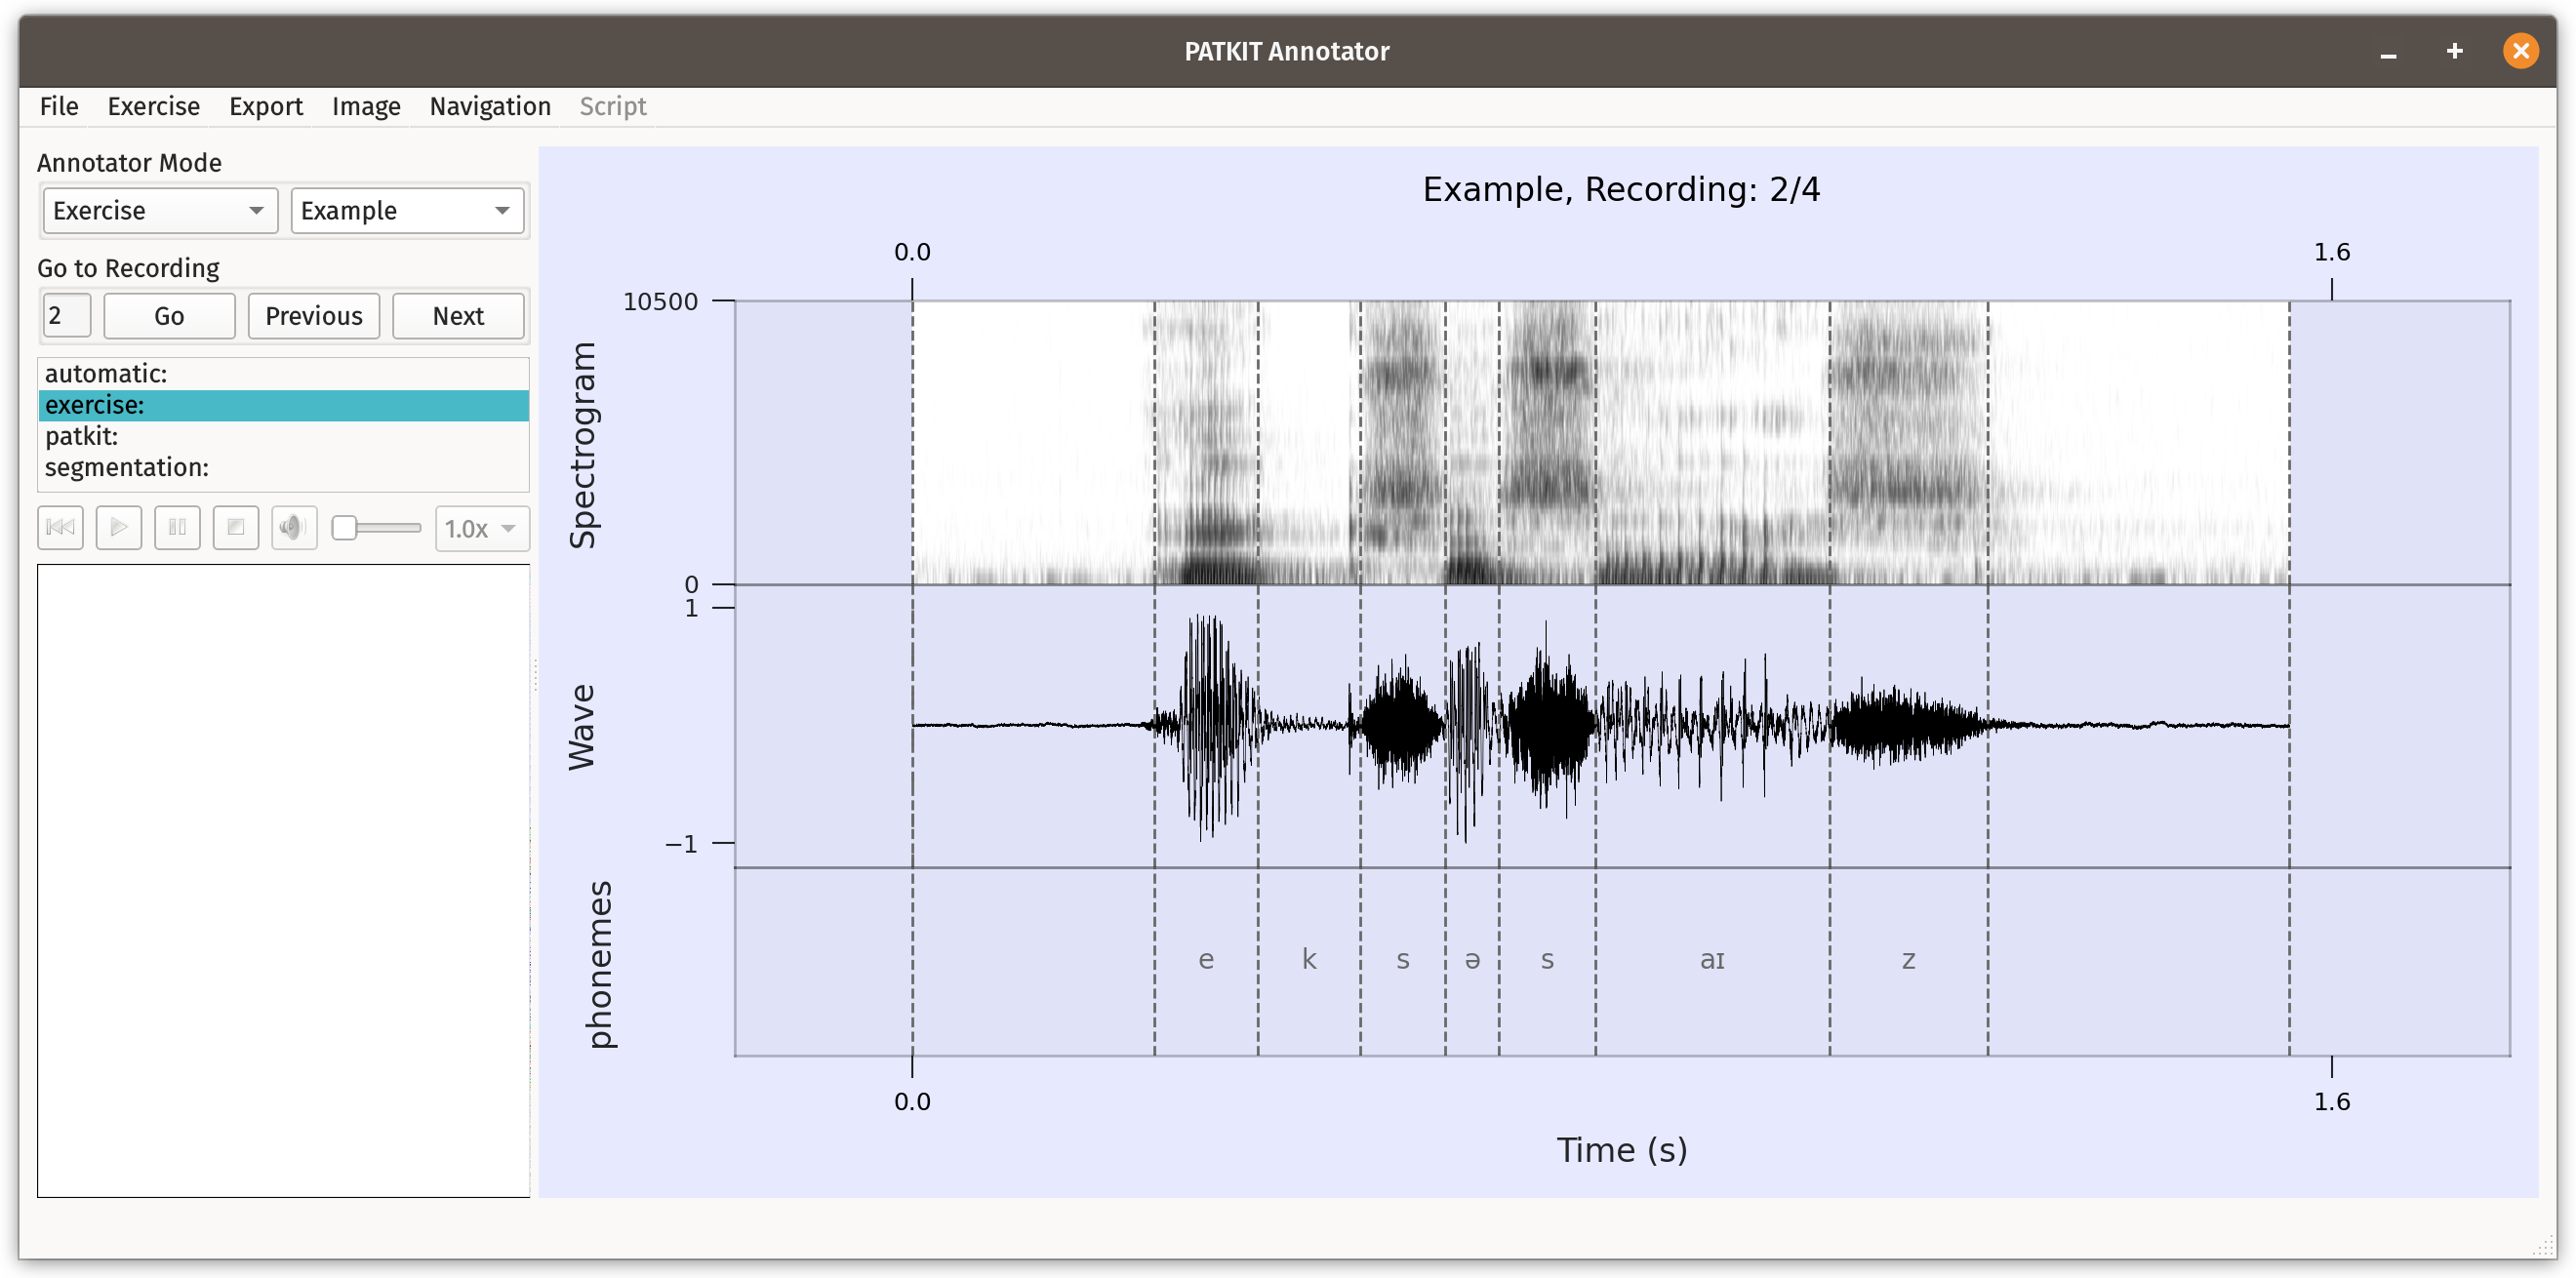
\includegraphics[width=\columnwidth]{patkit-example-3.png}
      \end{block}

      \begin{block}{User interface: Scrambled TextGrid}
          \centering
          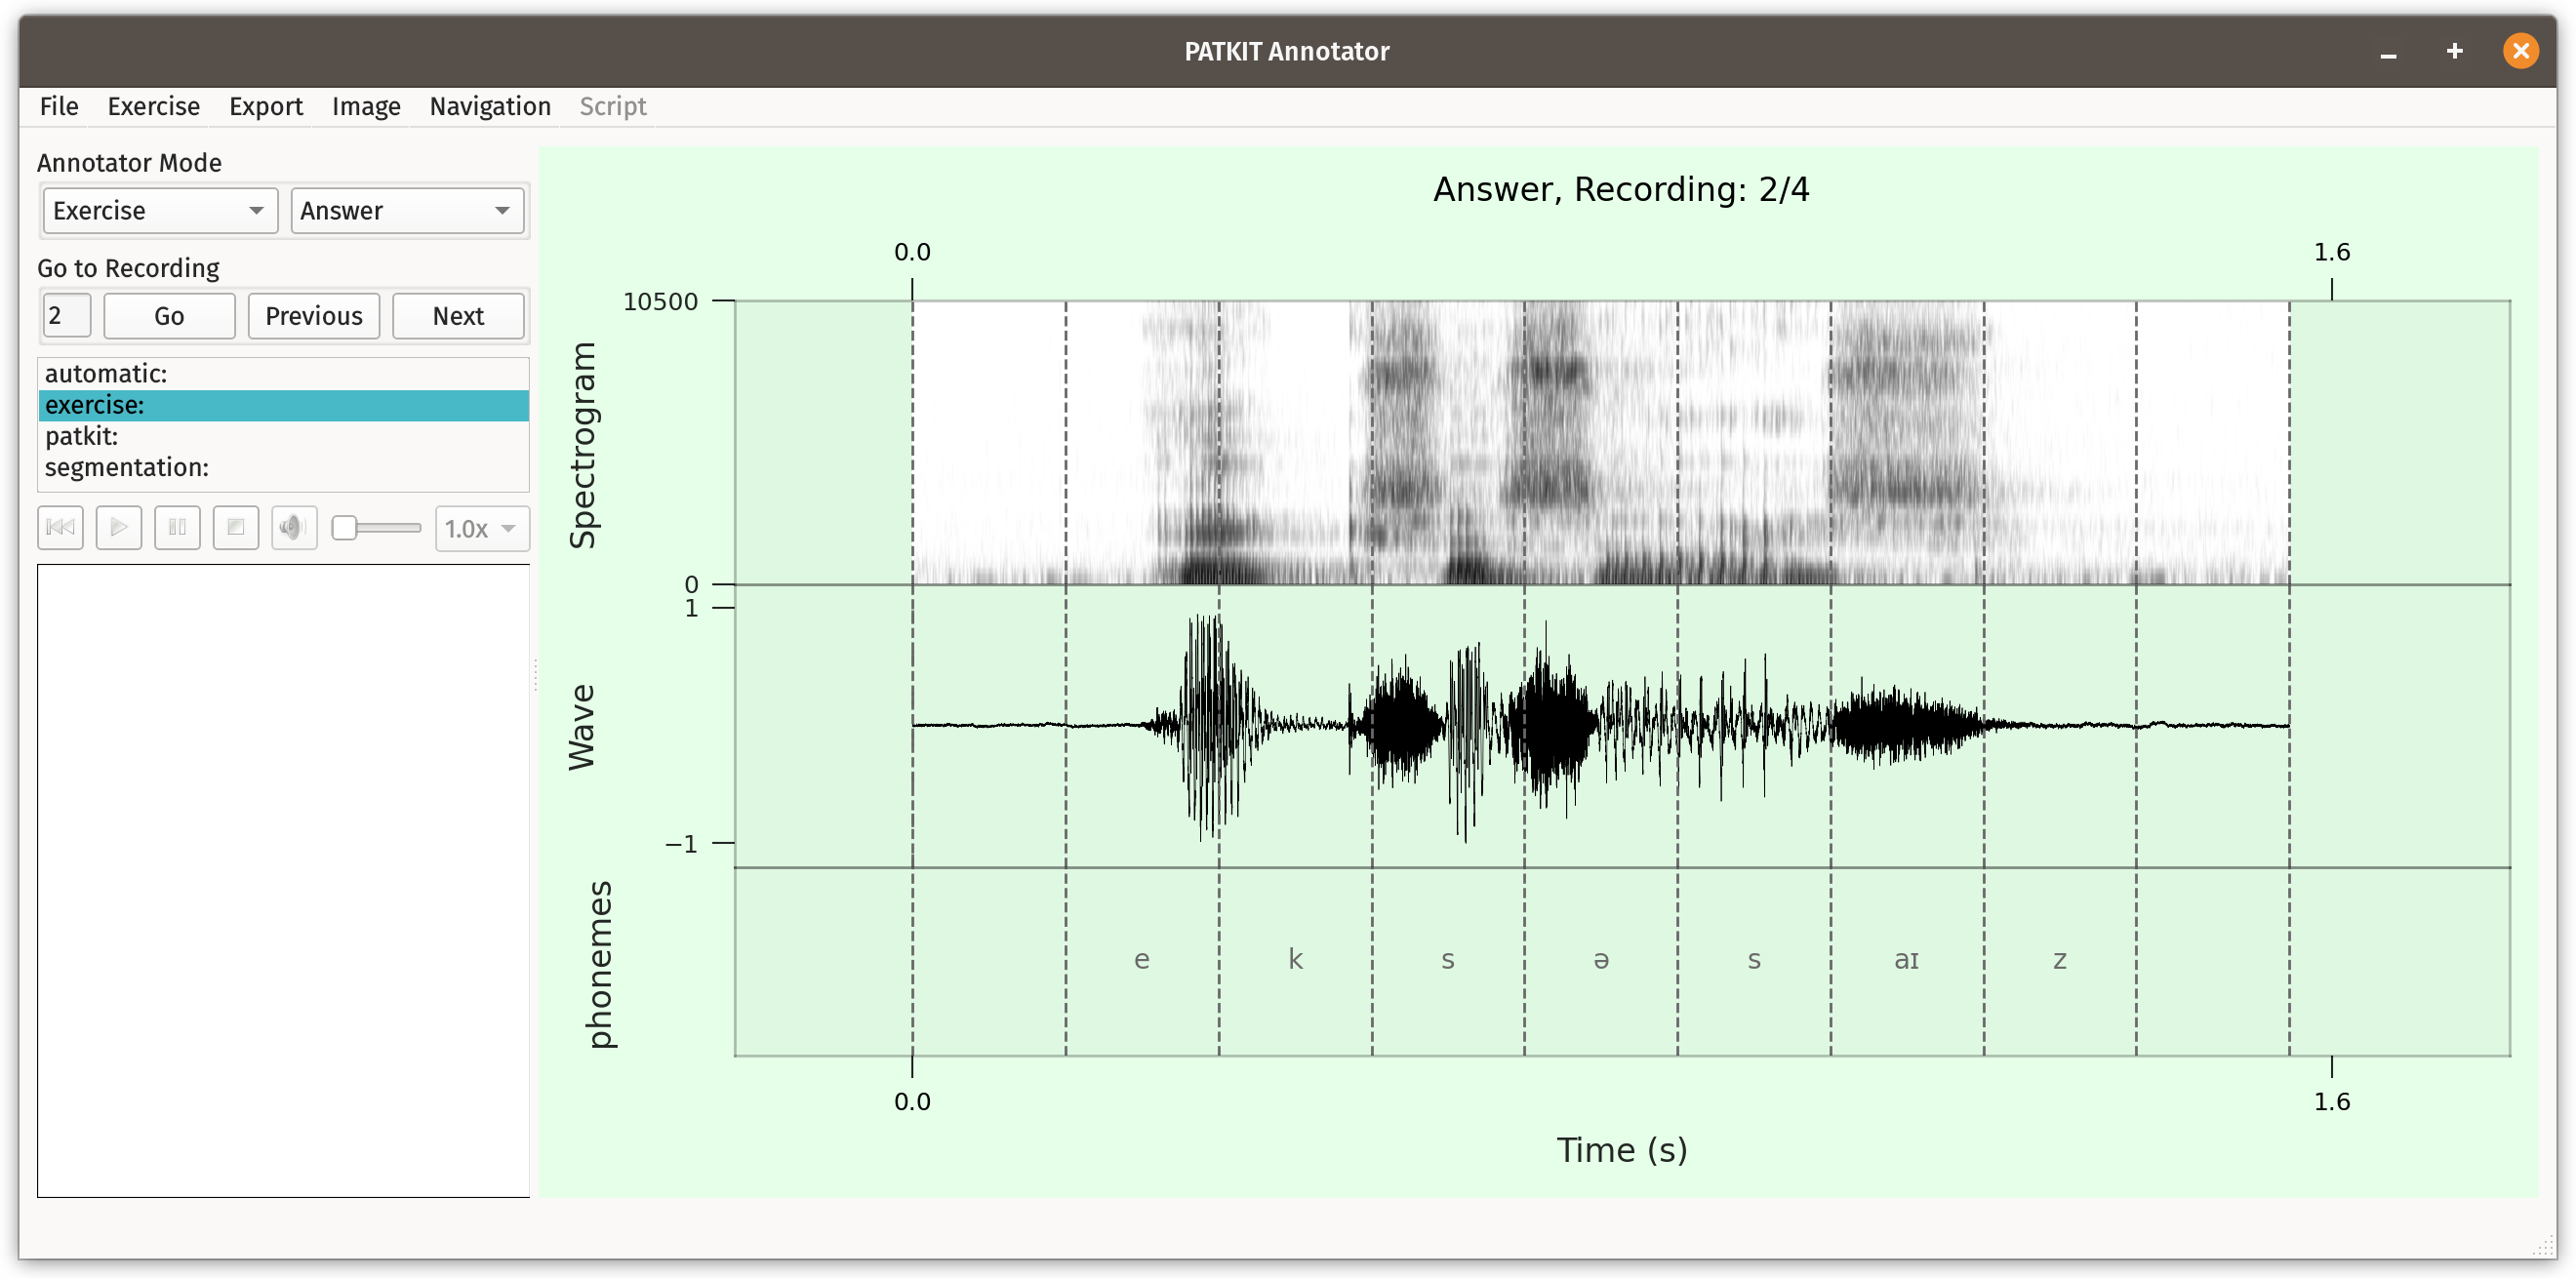
\includegraphics[width=\columnwidth]{patkit-answer-3.png}
      \end{block}

    \end{column}
  \end{columns}

  
\end{frame}


\end{document}

        % {Connection with speech cycling}
        % \begin{center}
        %   \includegraphics[width=.7\columnwidth]{Fowler_cycling}
        % \end{center}
        % \begin{itemize}
        % \item Figure from \cite{Fowler:NMC:1981}.
        % \item Metronome click at 0 ms.
        % \item Relevant intervals are: 1. silence between words, 3. onset
        %   consonant, and 4. vowel.
        % \end{itemize}

        % {Future work and questions}


%%%%%%%%%%%%%%%%%%%%%%%%%%%%%%%%%%%%%%%%%%%%%%%%%%%%%%%%%%%%%%%%%%%%%%%%%%%%%%%%%%%%%%%%%%%%%%%%%%%%
%%% Local Variables: 
%%% mode: latex
%%% TeX-PDF-mode: t
%%% End:
